\documentclass{article}
\usepackage[utf8]{inputenc}
\usepackage{lipsum}
\usepackage{authblk}
\usepackage{chngpage}
\usepackage{pdflscape}
\usepackage{paralist}

\usepackage[
  textwidth=18mm,
  textsize=tiny,
  linecolor=orange,
  colorinlistoftodos]{todonotes}

\title{Research and Implementation of Local Graph Transformations: Final report}
\author[1]{Kristóf Umann}
\author[1]{Miklós Vadász Dániel}
\affil[1]{Eötvös Loránd University, Faculty of Informatics}
\date{\today}

\input{preamble_tikz.tex}
\input{preamble_lstlisting.tex}

\begin{document}

\maketitle

\begin{abstract}
  Connected graphs are a natural choice of data structure to model overlay networks. A frequent problem overlay networks present is the adaptation of its topology towards an ideal topology. How the adoptation is performed is the subject of numerous academic papers -- we investigated and prototyped a novel approach that gracefully avoids sybil and eclipse attacks. The algorithm is discussed in a paper called \textit{,,On the complexity of local graph transformations''}\cite{ulgt}, and resticts the adaptation process' toolset to 4 well defined operations, or as the paper calls them, \textit{primitives}. The local graph transformation problem (\textit{LGT}) leans on the solution to the generalized undirected steiner forest problem (\textit{USF}). Both LGT and USF are NP-hard problems. \cite{ulgt} proposes a 2-approximate solution, and requires the use of a 2-approximate solution for USF.

  Our research and prototyping process presented unforeseen challenges and interesting results. On the research side, we found that clever root picking strategies can meaningfully reduce execution time and reduce the number of primitives needed to be used. We took measurements of our prototype that highlight how the number of primitives used and the execution time of the algorithm changes on graphs with different characteristics.
\end{abstract}

\section{Introduction}
\label{sec:introduction}

Connected graphs are a natural model of choice for overlay networks. A common characteristic of overlay networks is their ever changing nature: peers join and leave the network, a given connection might slow down or speed up. For this reason, there is frequent need to adopt the topology of the network towards a more ideal topology, for instance, to decrease the avarage file transfer time, or to avoid peers with too many or too few connections.

Studies explore this adaptation from the perspective of a supervisor that governs the network and removes or adds edges in the graph on its own, and from the perspective of peers, where the peers manage this process without a supervisor. Approaches employing a supervisor are efficient, but should they be malicious or faulty, they could lead the network vulnerable to sybil or eclypse attacks. Peer driven adaptations are generally slower, but are more resistent to these kinds of vulnerabilities.

\cite{ulgt} attempts to achieve a solution faster than the peer driven adaptation, while still being resistent to sybil and eclipse attacks. The idea is to have an entity knowledgable about the structure of the network, and calculate a list of operations that peers can perform to change the graph to a more ideal graph. An important aspect is that even despite the presence of a supervisor-like entity, the adoptation itself is done by the peers, and they can check whether the resulting graph would be malformed (hence the graph transformation being ,,local'').

This paper describes the analysis and prototyping of the undirected case of local graph transformations, or ULGT for short. In Section \ref{sec:ulgt}., we briefly overview the 2-approcimate ULGT algorithm presented in \cite{ulgt}. In Section \ref{sec:usf}., we discuss how a component of this algorithm, the \textit{Undirected Steiner Forest Problem}, was adjusted by us to work on non-edge weighted graphs. In Section \ref{sec:method}., we describe our measurement and statistic gathering methodology. We present the results of our research in Section \ref{sec:results}. Finally, we briefly discuss possibilities for further research in Section \ref{sec:future-work}.

\section{A brief overview of the ULGT algorithm}
\label{sec:ulgt}

ULGT restricts the set of operations that can be performed on the underlaying graph to 4 primitives. We demonstrate these primitives on Figure \ref{fig:primitives}., and describe them each below:

\textbf{Introduction} If a node $u$ has a reference of two nodes $v$ and $w$ with $v \neq w$, $u$ introduces $w$
to $v$ if $u$ sends a message to $v$ containing a reference of $w$ while keeping the reference.

\textbf{Delegation} If a node $u$ has a reference of two nodes $v$ and $w$ s.t. $u, v, w$ are all different,
then $u$ delegates $w$’s reference of $v$ if $u$ sends a message to $v$ containing a reference of $w$
and deletes the reference of $w$.

\textbf{Fusion} If a node $u$ has two references $v$ and $w$ with $v = w$, then $u$ fuses the two references
if it only keeps one of these references.

\textbf{Reversal} If a node $u$ has a reference of some other node $v$, then $u$ reverses the connection
if it sends a reference of itself to $v$ and deletes its reference of $v$.

\begin{figure}
  \centering
  \includegraphics[width=0.8\columnwidth]{primitives.png}
  \caption{The four primitives. For ULGT, the reversal primitive is not used.}
  \label{fig:primitives}
\end{figure}

We define ULGT as follows: given
two connected undirected graphs $G_s$, $G_t$, find a computation (a list of primitives to be applied in a sequence) of minimum length whose initial
graph is $G_s$ and whose final graph is $G_t$. Finding the ideal solution to ULGT is an NP-hard problem. As such, we're discussing a 2-approximate solution.

An important component we utilize is a solution to the \textit{(Generalized) Undirected Steiner Forest} problem (\textit{USF}). USF is defined as follows: For a given input $(G, S)$ such that $G$ is a graph and $S$ is a set of pairs of nodes from $G$, find a forest $F$ in $G$ with a minimum number of edges such that the two nodes of each pair in $S$ are connected by a path in $F$. USF is also NP-hard; we employ a 2-approximate solution to it.

We define the set of additional edges, $E_+$, as the set of edges present in $G_t$ but not in $G_s$. Similarly, the set of excess edges, $E_-$, is the edges present in $G_s$ but not in $G_t$. Following these definitions, the solution is split up to two parts: first, we calculate the list of primitives to be applied to $G_s$ to reach $G_s + E_+$, and second, we calculate the set of primitives to be applied to $G_s + E_+$ to reach $G_t$. The algorithm is demonstrated on Figure \ref{fig:ulgt-algorithm}.

\begin{figure}
  \textbf{Input:} Initial graph $G_s$ and final graph $G_t$.
  \vspace{1em}

  First part (add additional edges):
  \begin{compactenum}
  \item Compute a 2-approximate solution $F_{ALG,+}$ for the USF with input ($G_s$, $E_+$).
  \item For each tree T in $F_{ALG,+}$, select a root node $r_T$ and connect all nodes in $T$ that are incident to an edge in $E_+$ with $r_T$.
    \item For each ${u, v} \in E_+$, the root of the tree $u$ and $v$ belong to applies the introduction
  primitive to create the edge ${u, v}$.
  \item For each tree $T$ in $F_{ALG,+}$, delegate all superfluous edges (i.e., not belonging to $G_s$ or
  $E_+$) created during Step 2 bottom up in $T$ rooted at $r_T$ , starting with the lowest level.
  At each intermediate node fuse all of these edges before delegating them to the next
  parent.
  \end{compactenum}
  \vspace{1em}
  Second part (remove excess edges):
  \begin{compactenum}
  \item Compute a 2-approximate solution $F_{ALG,-}$ for the USF with input $(G_t, E_-)$.
    \item For each $e \in E_-$, let $s(e)$ be an arbitrary of the two endpoints of $e$. For each tree $T$
    in $F_{ALG,-}$, select a root node $r_T$ and for each $e \in E_-$ whose endpoints belong to $T$,
    connect $s(e)$ with $r_T$.
    \item For each $e \in E_-$, $s(e)$ delegates $e$ to $r_T$.
    \item For each tree $T$ in $F_{ALG,-}$, delegate all superfluous edges (i.e., not belonging to $G_t$)
  bottom-up while fusing multiple edges as in Step 4 of the first part.
  \end{compactenum}
  \caption{Approximating algorithm for ULGT}
  \label{fig:ulgt-algorithm}
\end{figure}

\cite{ulgt} is vague in terms of which $r_T$ root we pick for either of the two parts of the algorithm. Upon research, we concluded that for the second part, if all nodes in the steiner trees participate in $S$, a root outside the tree must be picked. The reason behind this is that the delegation primitive demands three different nodes, and the meaning of every node in the tree participating in $S$ is that every node must be a part of at least one delegation operation. However, our experimentation showed that this is an exceptional case, and for the overwhelming majority of steiner trees we are able to pick this root inside the steiner tree. This way, we saved at least one introduction primitive to connect a node outside the tree to it.

\section{Adjusting a 2-approximate USF algorithm for non-weighted graphs}
\label{sec:usf}

On the account of the USF problem we leaned on Yossi Azar's algorithms lecture notes~\cite{usf}. The subject of this algorithm however is an edge-weighted graph. Since the input of ULGT is a non-edge weighted graph however, we adjusted the algorithm to work on an edge \textit{labels}. We define the set of labels $L$ on $(u,v)$ as follows:
\begin{itemize}
  \item $ConnectsMM$\footnote{$M$ stands for \textit{Marked}, a term used in our prototype's source code.}: if both $u$ and $v$ participate in $S$.
  \item $ConnectsMNM$: if one and only one of $u$ or $v$ participates in $S$.
  \item $ConnectsNMNM$: if neither $u$ nor $u$ participate in $S$.
\end{itemize}

A fundamental element of the 2-approximate USF algorithm is edge contraction. Upon contracting $(u,v)$, we form a new node $n$ that represents both $u$ and $v$, meaning that if either $u$ or $v$ participates in $S$, $n$ participates in $S$. With that said, we present our adjusted algorithm on Figure~\ref{fig:usf-algorithm}.

\begin{figure}
  \textbf{Input:} An undirected graph $G = (V, E)$, a weight function $c : E \rightarrow L$ and a set of node pairs $S = \{(a, b) | a, b \in V \}$.

  \textbf{Solution:} A forest $G' = (V', E')$ with minimal number of edges, in which $\forall (s_i, t_i) \in S$ there is a path from $s_i$ to $t_i$.
  \vspace{1em}

  Let us define $A = \{u | (u=s_i \vee u = t_i) \wedge s_i \neq t_i\}$, the set of vertices that have not yet been contracted with
  their pair.
  \vspace{1em}

  \textbf{The algorithm:}
  \begin{compactenum}
  \item For each edge $(u,v) \in G$, and upon reaching the last edge, start over from the first:
    \begin{compactenum}
      \item If $c(u,v) = ConnectsMM$, we contract $(u,v)$. If $A = \emptyset$, exit the loop.
      \item Recalculate edge weights.
    \end{compactenum}
  \item Drop all non-contracted edges. Uncontract contracted edges.
  \item Drop edges that don't participate in the shortest path from $(u, v)$, for all node pairs in $S$.
  \item Drop edges that close a cycle.
  \end{compactenum}
  
  \caption{Approximating algorithm for USF}
  \label{fig:usf-algorithm}
\end{figure}

Our adjustments elegantly avoids the problem of needing integer, or worse, floating point values to represent edge weights, and allows for strong type enforcement with the use of enumerating classes, without any performance loss.
%\section{Implementation}
%We prototyped both ULGT and USF in a C++ program, written without the use of third party libraries. While this presented a sizable setback in our implementation, it also allowed us to tailor our graph implementation to fit the problem better. 
\section{Measurement methodology}
\label{sec:method}

Our interest centered around two metrics: the \textit{execution time} of the algorithm and the \textit{number of primitives} to be applied. Upon reserching \cite{ulgt}, we identified three elements that affect these:
\begin{itemize}
  \item The input graph $G_s$: the number of nodes and the number of edges. One another important aspect is the structure; suppose you have a node that is connected to every other node while the rest of the nodes have very few neighbours, or suppose that each node is relatively even in terms of number of neighbours.
  \item The number of additional edges.
  \item The number of excess edges.
\end{itemize}

We implemented a connected graph generating algorithm with four parameters: the graph size, edge densitiy (how many neighbours a node should have on average), the number of excess and the number of additional edges.

We found that we needed to use several independent pseudo-random number generators to measure the change of a single parameter with satisfactory accuracy. Should we generate more edges by increasing edge density, we want the placement of additional edges to change as little as possible. We also needed to avoid the same edge being present in both the set of additional and excess exdes -- this, while we needed to preserve the connectivity proved to be a challange, and we decided to skip the generation of an edge if it proved too difficult. The implication is that the generated graph may not have the same parameters as was requested from the graph generator. However, we took our measurements on the actual metrics of the graph, not the the generation parameters, so our results aren't impeded by this issue.

While we're confident in our adjustments to the USF algorithm are beneficial, we struggled to find an efficient solution, something that required changes to our measurement methodology. The run time of our USF implementation was several order of magnitude longer than the rest of the code. Because of this, it was difficult to find parameters for graph generations that meaningfully measured, on the computing resources available to us, the runtime of USF, and ULGT without USF.

For this reason, we decided to again adjust the USF algithm, skipping the edge contraction and uncontraction stage. As seen on Figure~\ref{fig:usf-algorithm}., the resulting forest would be composed of the shortest paths in between the node pairs in $S$. This would certainly satisfy the requirement that each node pair must lie on the same tree, but the resulting forest would on occation be larger than the authentic USF algorithm. Therefore, we can no longer claim that our implementation is a 2-approximate USF algorithm, as required by the ULGT algorithm. However, since neither the 2-approximate nor our adjusted solution is necessirily optimal, we feel our measurements of ULGT excluding the runtime of our USF solution are still statistically relevant.

With that said, we took measurements of our USF algorithm that includes the edge contraction/uncontraction parts on graph generated with smaller parameters.

We also made sure to measure the meaningful parts of our algorithm, ignoring any I/O operations and avoided running background applications whenever possible.

\section{Results}
\label{sec:results}

We collected several different kinds of data on our prototype, such as the runtime of the entire algorithm, runtime of our USF solution in both the 2-approximate and further adjusted configuration, data on our root picking strategy, the number of different primitives used, the number of steiner trees produced, and the actual metrics of the generated input graphs $G_s$ and $G_t$. Here, we present those that we found statistically significant.

Note that numbers don't steadily increase or descrease as one would expect. This is a result of the randomness of our graph generation algorithm. We display the execution time of our implementation of the 2-approximate USF solution for each of the 3 classes of graph typed we measured, but we are not confident whether we can draw conclusions from it until we get the chance to implement a more efficient solution.

On Figure~\ref{fig:edge-density}, we demonstate correlation in between increasing edge density and the execution of ULGT without the USF parts. We found that a graph whose nodes have evenly few edges require many more primitives than ,,denser'' graphs, but their count are relatively consistent after a treshold density is reached. We also found that on every graph, if the size of the set of excess and addition edges where the same, the number of addition, delegation and fusion primitives remained the same. The latest version of our USF algorithm yielded the most amount of steiner trees when each node was neighbouring 10\% of the nodes in the graph, and had fewer in denser graphs.

On Figure~\ref{fig:additional-edges}, we show a graph indicating correlation in between the runtime of ULGT and increasing number of additional edges. Expectedly, we show a strong correlation in between the number of primitives used and increasing additional edge count (note that the orange line represents either the count of delegation and fusion primitives, as their count was the same). The number of steiner trees briefly increased and topped around 120 additional edges, and drops all the way to 1. This makes sense; when every node participates in $S$, a spanning tree would the solution to USF.

Figure~\ref{fig:excess-edges} demonstrated similar results to the one shown on Figure~\ref{fig:additional-edges}, but seems to drop in the number of steiner trees far sharper with increasing edge density.

\begin{landscape}
\begin{figure}
  \vspace{-1.7cm}
  \centering
  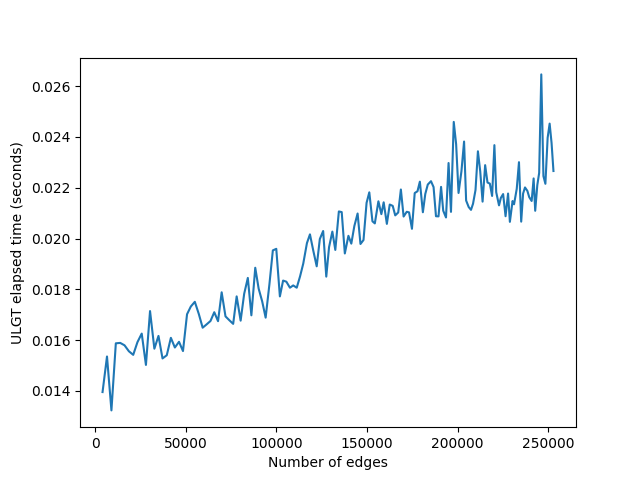
\includegraphics[width=0.48\columnwidth]{figures/edge_density_time.png}
  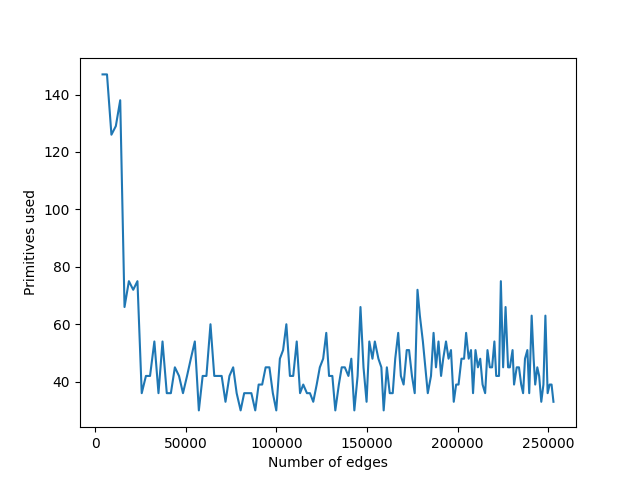
\includegraphics[width=0.48\columnwidth]{figures/edge_density_primitive_count.png}
  
  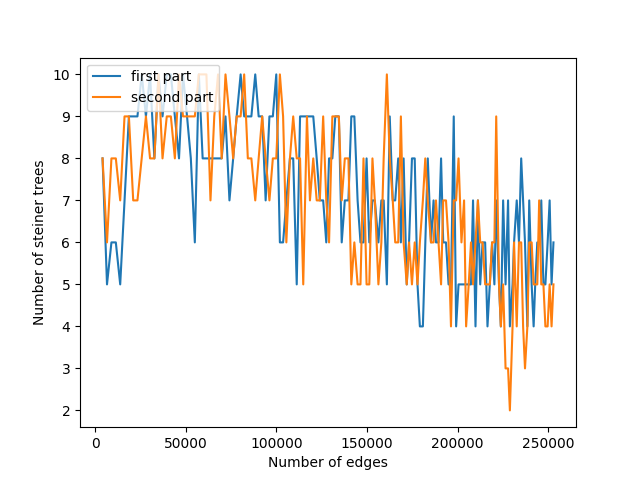
\includegraphics[width=0.48\columnwidth]{figures/edge_density_steiner_tree_count.png}
  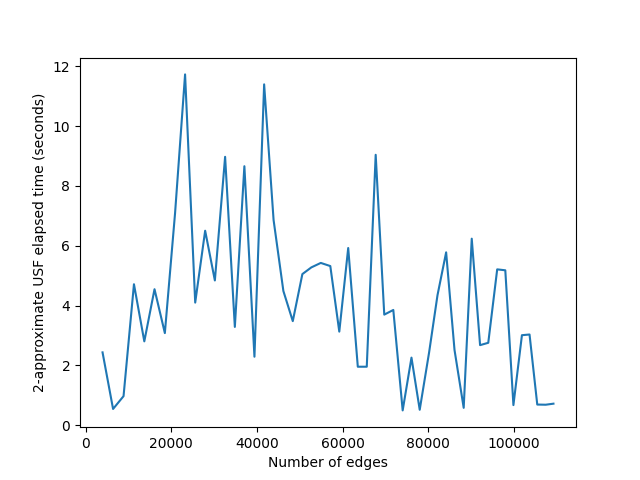
\includegraphics[width=0.48\columnwidth]{figures/edge_density_contraction_time.png}

  \caption{Measurements on increasing edge density. All graphs had 1000 nodes, and there were 10 additional and 10 excess edges.}
  \label{fig:edge-density}
\end{figure}
\end{landscape}

\begin{landscape}
\begin{figure}
  \vspace{-1.7cm}
  \centering
  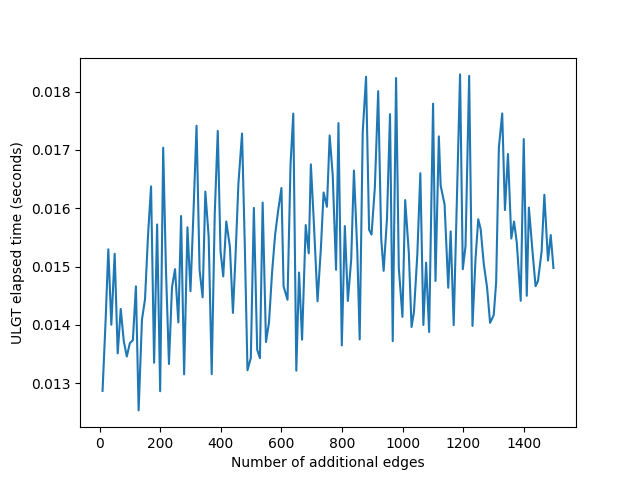
\includegraphics[width=0.48\columnwidth]{figures/additional_edge_time.png}
  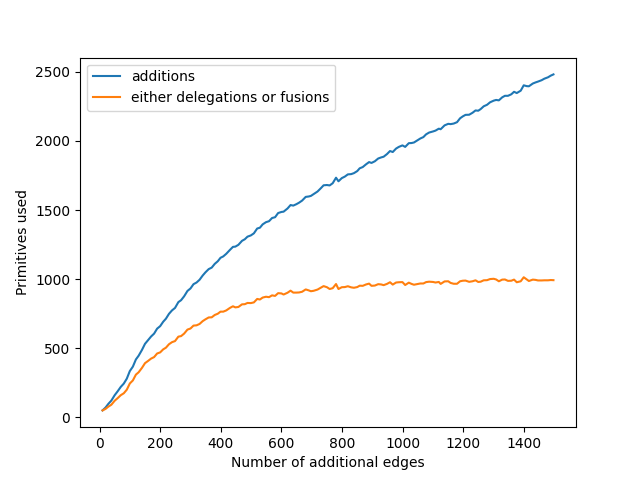
\includegraphics[width=0.48\columnwidth]{figures/additional_edge_primitives.png}
  
  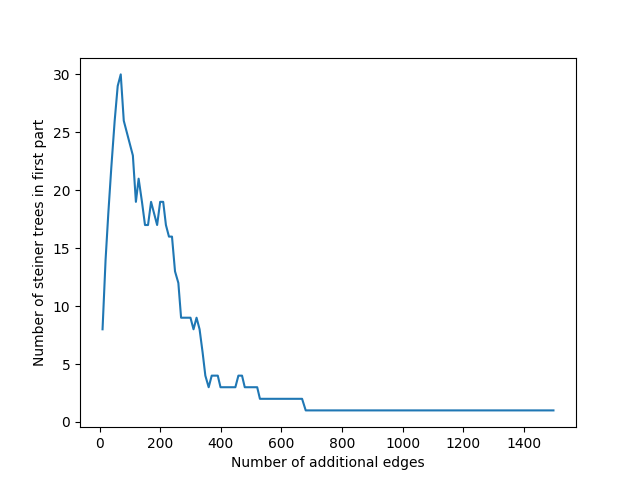
\includegraphics[width=0.48\columnwidth]{figures/additional_edge_steiner.png}
  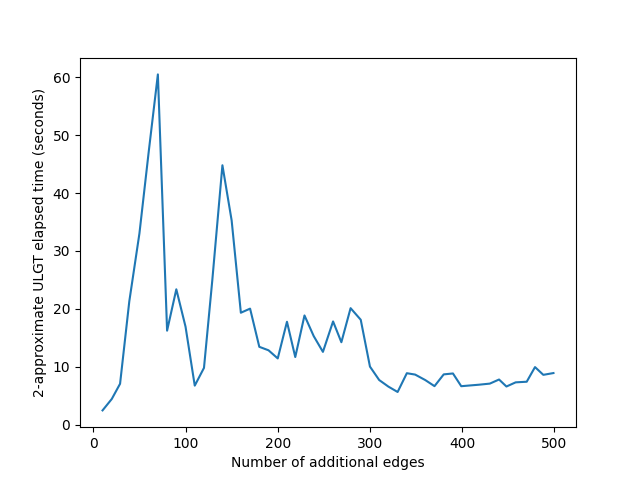
\includegraphics[width=0.48\columnwidth]{figures/additional_edge_contraction_time.png}

  \caption{Measurements on increasing additional node count. All graphs had 1000 nodes, had the edge density set to 5, and had 10 excess edges.}
  \label{fig:additional-edges}
\end{figure}
\end{landscape}
  
\begin{landscape}
\begin{figure}
  \vspace{-1.7cm}
  \centering
  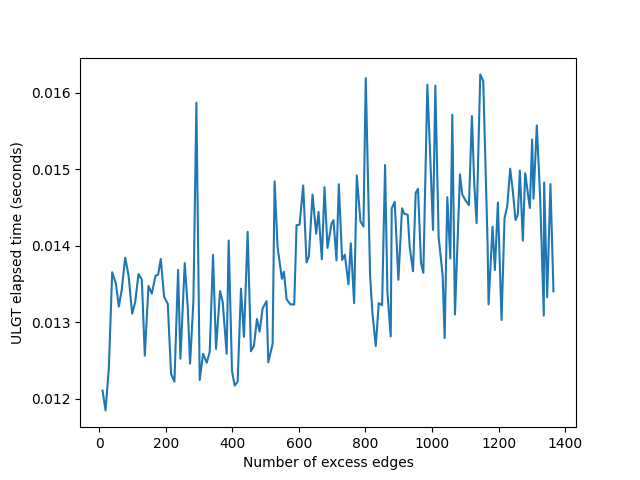
\includegraphics[width=0.48\columnwidth]{figures/excess_edge_time.png}
  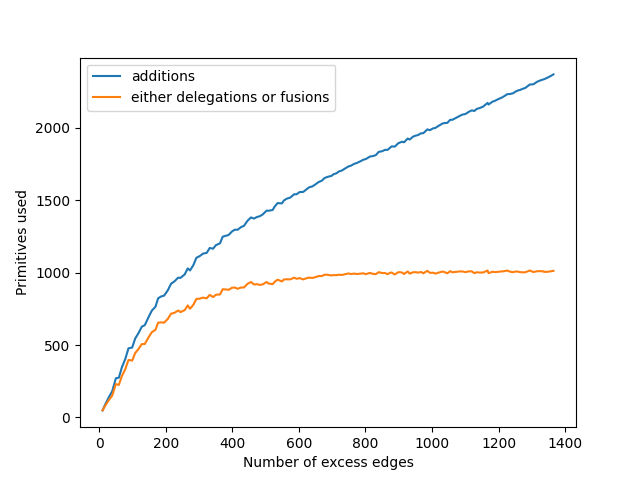
\includegraphics[width=0.48\columnwidth]{figures/excess_edge_primitives.png}
  
  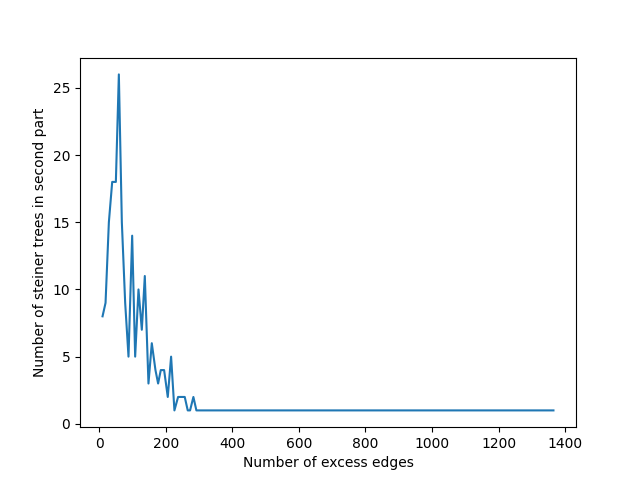
\includegraphics[width=0.48\columnwidth]{figures/excess_edge_steiner.png}
  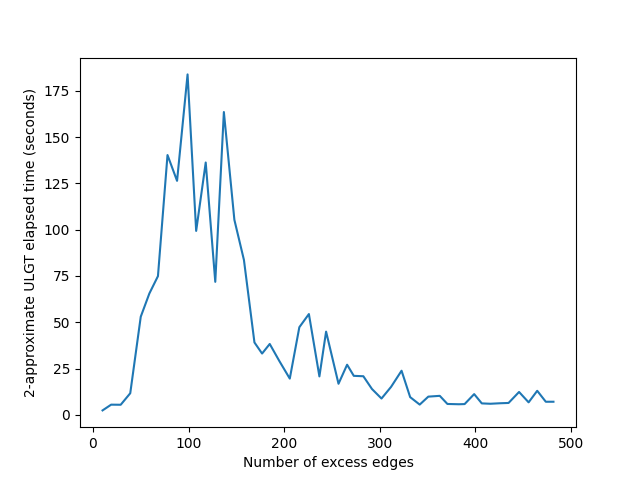
\includegraphics[width=0.48\columnwidth]{figures/excess_edge_contraction_time.png}

  \caption{Measurements on increasing excess node count. All graphs had 1000 nodes, had the edge density set to 5, and had 10 additional edges.}
  \label{fig:excess-edges}
\end{figure}
\end{landscape}

Despite running our algorithm on 250 different graphs, no cases were found where we needed to pick a root outside a steiner tree.

\section{Future work}
\label{sec:future-work}

We mentioned the structure of the graph as a possible contributing factor the number of used primitives and execution time of the algorithm. We experimented with so called ,,mega nodes'' that have several times more neighbours than the rest of the nodes, we realized that in order to reap the benefits of such a structure, we might need a better root picking strategy.

Generally speaking, we think there is room for improvement on choosing the optimal root. Maybe if we tried to pick the one with the highest amount of neighbors we could reduce the number of introduction primitives needed.

While our research on conducting USF on a non-edge weighted graph is primising, we didn't have the time to implement a solution that displays this. We have some ideas that could bring the execution time to be in line with the rest of the ULGT runtime.

\cite{ulgt} itself mentions that although this is a novel approach to avoid sybil or eclipse attacks resulting from a malicious or malfuncioning supervisor, the same can't be said if the peers themselves. Further research on this front would be interesting, especially the performance impact that the increased security would bring.

\section{Conclusion}

Overlay networks frequently need to adopt their topology towards a more ideal topology. Superviros driven solutions leaves the network vulnerable to sybil and eclipse attacks. Peer driven solutions are inefficient. The paper called ,,On the complexity of local graph transformations'' presents an elegant solutions that is resistent to either of these vulnerabilites, while still being more efficient then a peer driven approach. To achieve this, it defines four graph transforming primitives, and a 2-approximate solution to calculate the list of primitives to be applied to a starting graph to construct a more ideal graph.

We researched and prototyped the undirected version of the 2-approximate solution. We also implemented an algorithm that is a part of the solution, called the generalized undirected steiner forest problem. We managed to find ways to improve on the number of primitives necessary for the 2-approximate solution with a clever root picking strategy, and proposed ideas for further improvements. The 2-approximate steiner forest solution, which was designed for edge-weighted graphs, was adjusted to work on edge-labeled graphs, easily contructible in the absence of edge weights. Though we found it challenging to implement this algorithm after all, we demonstated how to take meaningful measurements with further adjustment even with limited computing resources.

We showed strong correlation in the execution time if either the edge count, the number of excess or number of additional edges increase. We showed that the number of primitives needed decrease only to a point with with increasing edge count. We also highlighted future research opportunities that center around graph adoptation.

\bibliographystyle{IEEEtran}
\bibliography{IEEEabrv,references}

\end{document}

